Для разработки процессорной системы существует возможность использовать готовые блоки, предоставляемые компанией - производителем Xilinx. В данной работе используются некоторые из них. Также для передачи комманд и параметров оператора был разработан пользовательский блок виртуальных регистров. Список всех блоков и их краткое описание представлены в таблице()\par
\begin{table}
    \caption{Блоки дизайна процессорной системы}
   % \begin{tabular}{|>{\centering\arraybackslash}p{0.45\textwidth}|>{\centering\arraybackslash}p{0.45\textwidth}|}
    \begin{tabular}{|p{0.45\textwidth}|p{0.5\textwidth}|}
        \hline
        Наименование блока & Описание \\
        \hline
        Процессорная система ZYNQ7 Processing System & Программный интерфейс вокруг процессорной системы платформы Zynq-7000 \\
        \hline
        Контроллер блоков памяти AXI BRAM Controller & Является конечным ведомым модулем для интеграции с интерфейсом шины AXI и системными главными устройствами для связи с локальными блоками оперативной памяти \\
        \hline
        Интерфейс шины AXI Interconnect & Соединяет один или более AXI устройств, отображенных на память в режиме мастера, к одному или более устройствам, отображённых на память в режиме ведомого \\
        \hline
        Сброс процессорной системы Processor System Reset & Обеспечивает индивидуальные сбросы для всей процессорной системы, включая процессор и переферийные устройства \\
        \hline
        Интерфейс модуля виртуальных регистров reg\_interface & Пользовательский блок, использующий интерфейс AXI4-Lite \\
        \hline
        Генератор блоков памяти Block Memory Generator & Автоматизирует создание блочных запоминающих устройств для программируемой логики\\
        \hline
    \end{tabular}
\end{table}
Как видно из приведённой таблицы, в процессорной системе используется несколько готовых блоков от компании Xilinx и один пользовательский модуль, который имеет смысл рассмотреть подробнее. Он разработан с использованием AXI4-Lite --- данного интерфейса хватает для корректной работы модуля в силу небольшого объёма данных, передаваемых за одну транзакцию. Задача блока reg\_interface заключается в передаче коротких параметров, комманд и сигналов подтверждения из процессора в программируемую логику. Сигналы модуля представлены на рисунке().\par 
\begin{figure}[ht]
    \centering
    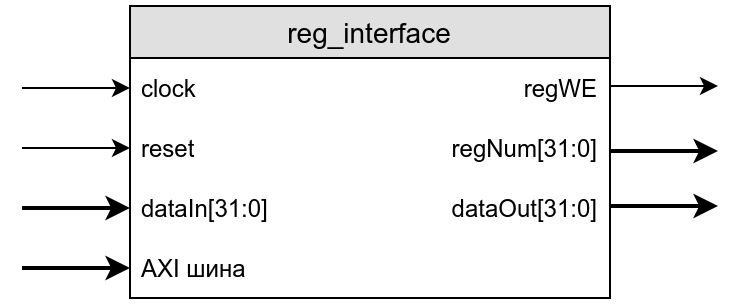
\includegraphics[width=0.5\linewidth]{reg_interface.png}
    \caption{Сигналы блока reg\_interface}
    \label{fig:mpr}
\end{figure}
Каждый пользовательский сигнал (dataPLtoPS, regWE, regNum, dataPStoPL) ассоциирован с определённым участком в памяти, таким образом, текущее значение по выбранному адресу является состоянием сигнала. Блок модуль связан с модулем reg\_file программируемой логики, подробное описание которого будет приведено в соответствующей главе. Сейчас важно то, что этот модуль содержит виртуальные регистры; операции с ними осуществляются посредством рассматриваемого модуля reg\_interface, который переводит их в операции с реально существующими регистрами.\par
Для записи в виртуальный регистр необходимо вставить данные в сигнал dataPStoPL, затем установить номер регистра в сигнал regNum, после чего подать единицу в сигнал regWE.\par
Для чтения из виртуального регистра необходимо установить номер интересующего регистра в сигнал regNum, после считать данные из сигнала dataPLtoPS.\par
Общая диаграмма блоков процессорной системы изображена на рисунке().\par
\begin{figure}[ht]
    \centering
    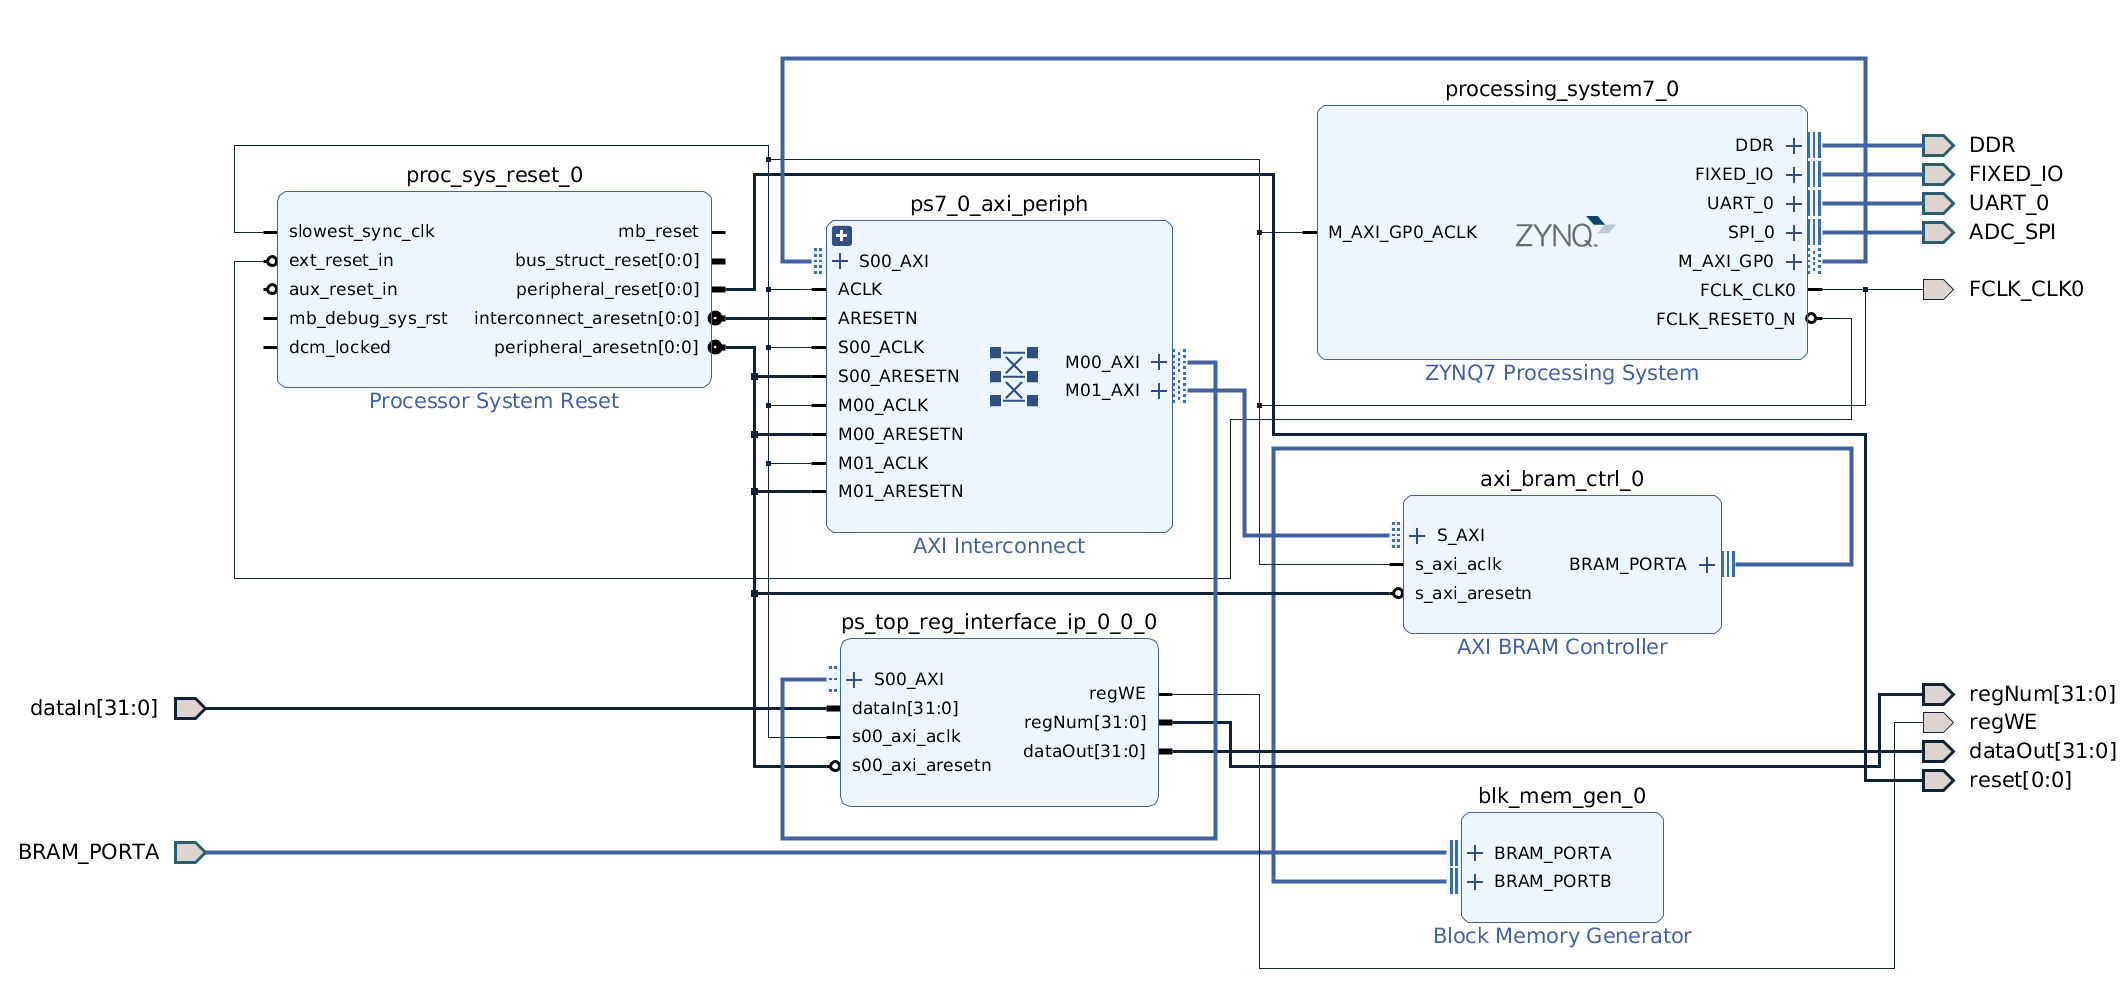
\includegraphics[width=1\linewidth]{ps_top.jpg}
    \caption{Диаграмма блоков процессорной системы}
    \label{fig:mpr}
\end{figure}
Кроме интерфейса виртуальных регистров, рассмотренного выше, для обмена данными между процессорной системой и программируемой логикой используется модуль двухпортовой памяти blk\_mem\_gen\_0: через порт A происходит запись данных из программируемой логики, а черех порт B информация считывается и отправляется в процессор. Данный модуль предназначен для передачи экспериментальных данных для их последующего отображения оператору стенда.
